\section{Problem geometry and experimental setup}
\label{sec:experiments}

\begin{figure}[htbp]
    \centering
    % \begin{tikzpicture}[
    % axPic/.pic={
    %         \draw[->,-triangle 45] (0,0) -- (-0.15,1)  node (ysign) [pos=1,right] {$y$};
    %         \draw[->,-triangle 45] (0,0) -- (0.9,0.27) node (xsign) [pos=1,right] {$x$};
    %         \draw[->,-triangle 45] (0,0) -- (0.6,-0.2) node (zsign) [pos=1,right] {$z$};
    %         \node[font=\scriptsize,xshift=0.4cm]  at (ysign.north) {{(transverse)}};
    %         \node[font=\scriptsize,xshift=0.48cm] at (xsign.south) {{(streamwise)}};
    %         \node[font=\scriptsize,xshift=0.4cm]  at (zsign.south) {{(spanwise)}};
    %      }
    % ]
    %     \node (0,0) (geomFig) {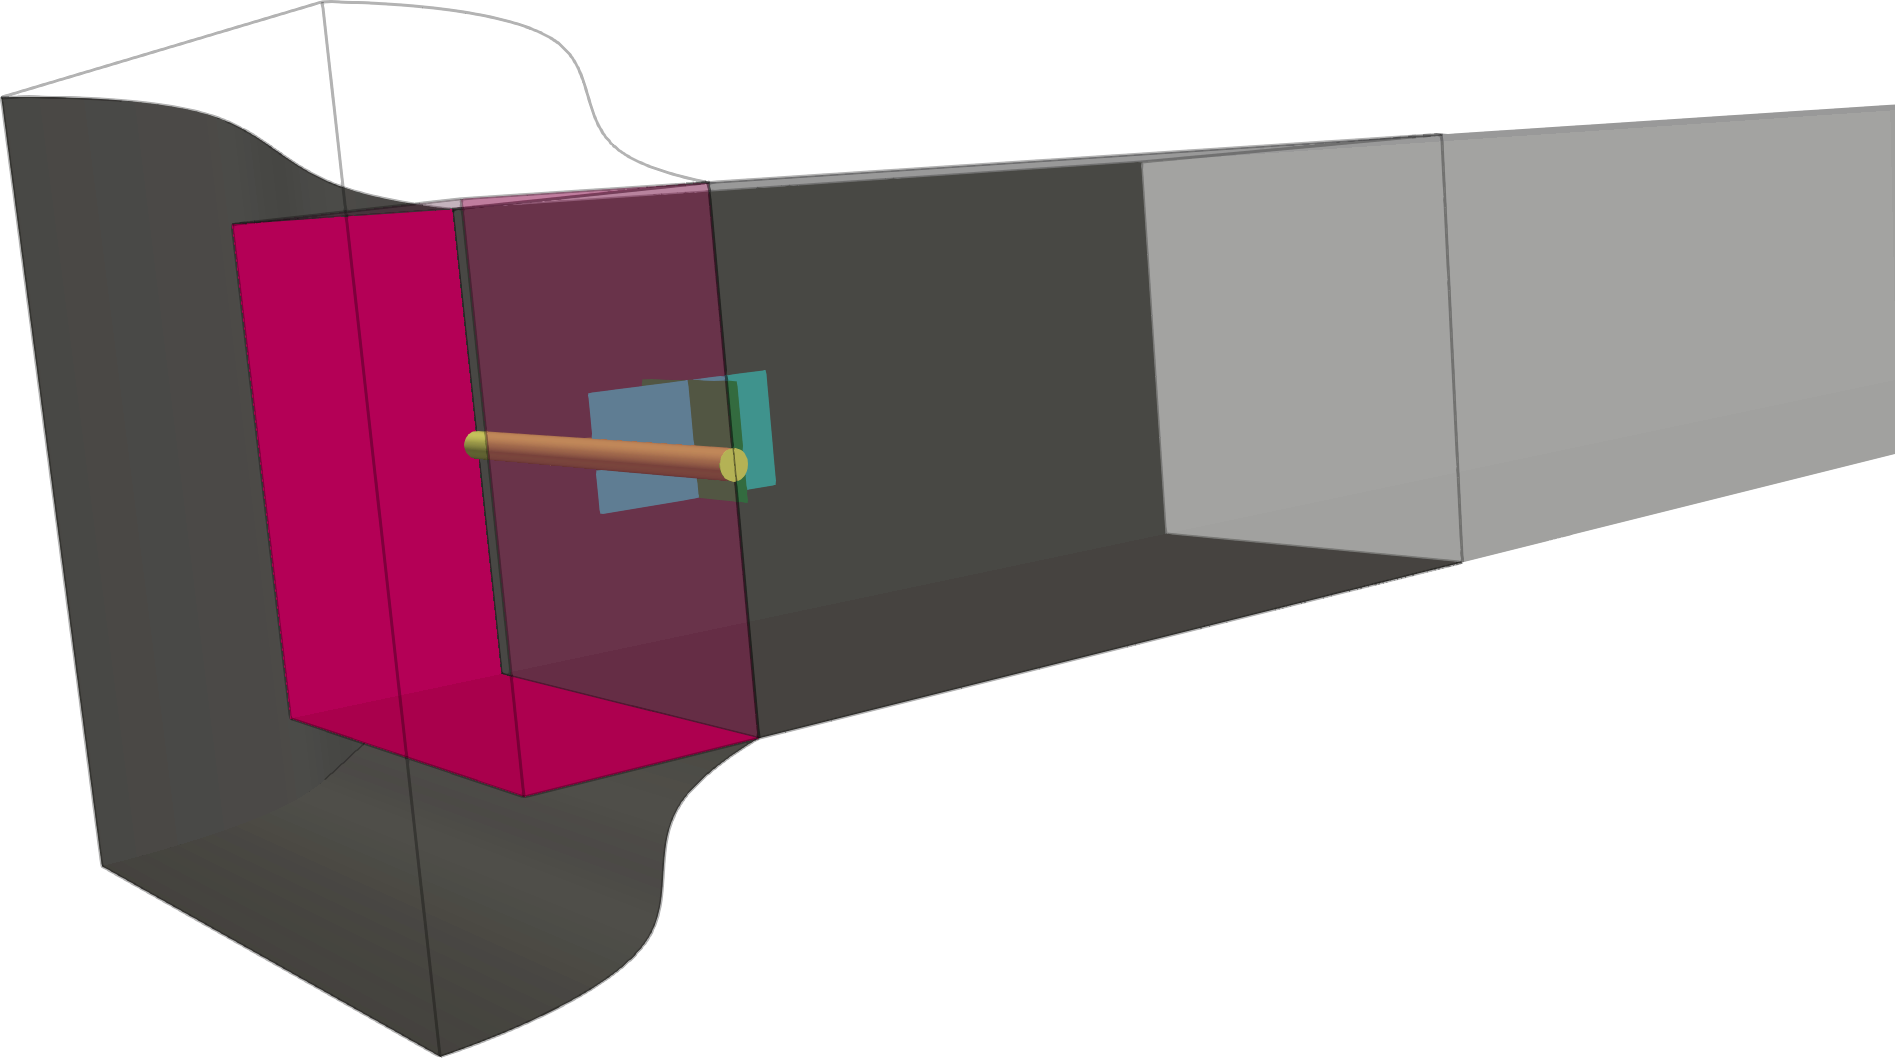
\includegraphics[width=0.9\textwidth]{\myImages/windTunnelFullV2.png}};
    %     \node[anchor=south east] (cylFig) at (geomFig.south east) {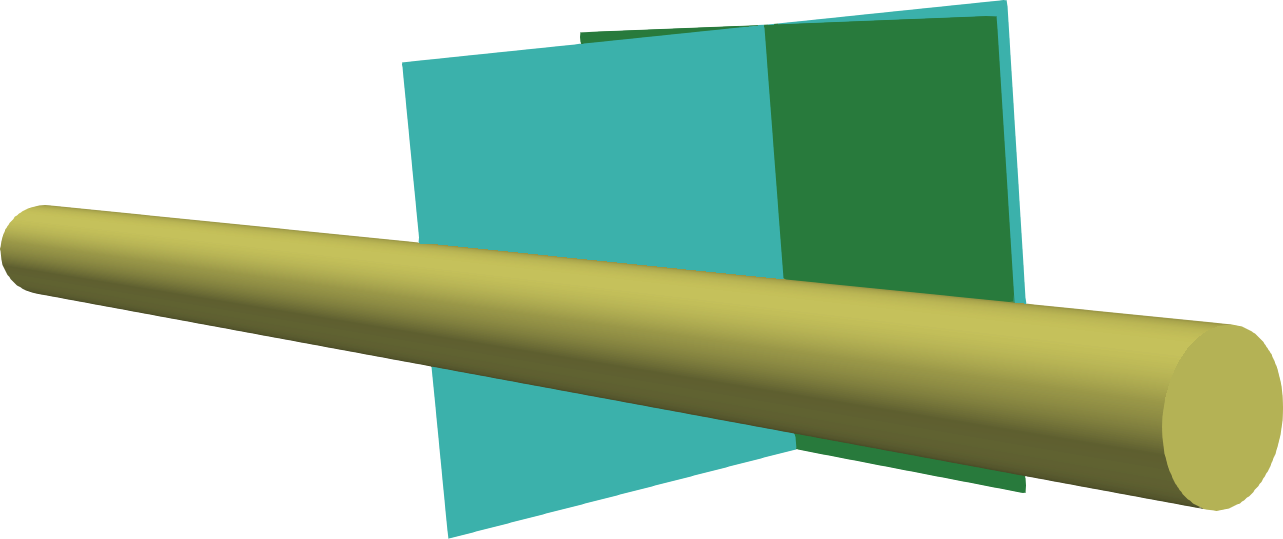
\includegraphics[width=0.45\textwidth]{\myImages/cyllAndPoMsV3.png}};
    %     \node[anchor=north,below left=0.3cm and 1cm] at (geomFig.north) {a)};
    %     \node[anchor=north west,below right=0.3 and 0.3cm] at (cylFig.north west) {b)};
    %     \draw (-1.3,-3) pic[solid] {axPic};
    %     \draw[->,-triangle 45,thick, red!80!black] (-0.5,-2.5) -- (1.1,-2.05) node[pos=0.2,above]{$\bm{u}_{\mathrm{in}}$};
    %     \draw[->,teal!70!white,thick] (1,-1.1) -- (1.7,-1.5) node[pos=0.2,above]{PoM1};
    %     \draw[->,green!70!black,thick] (5,-1.1) -- (4,-1.5) node[pos=0.0,above]{PoM2};
    % \end{tikzpicture}
    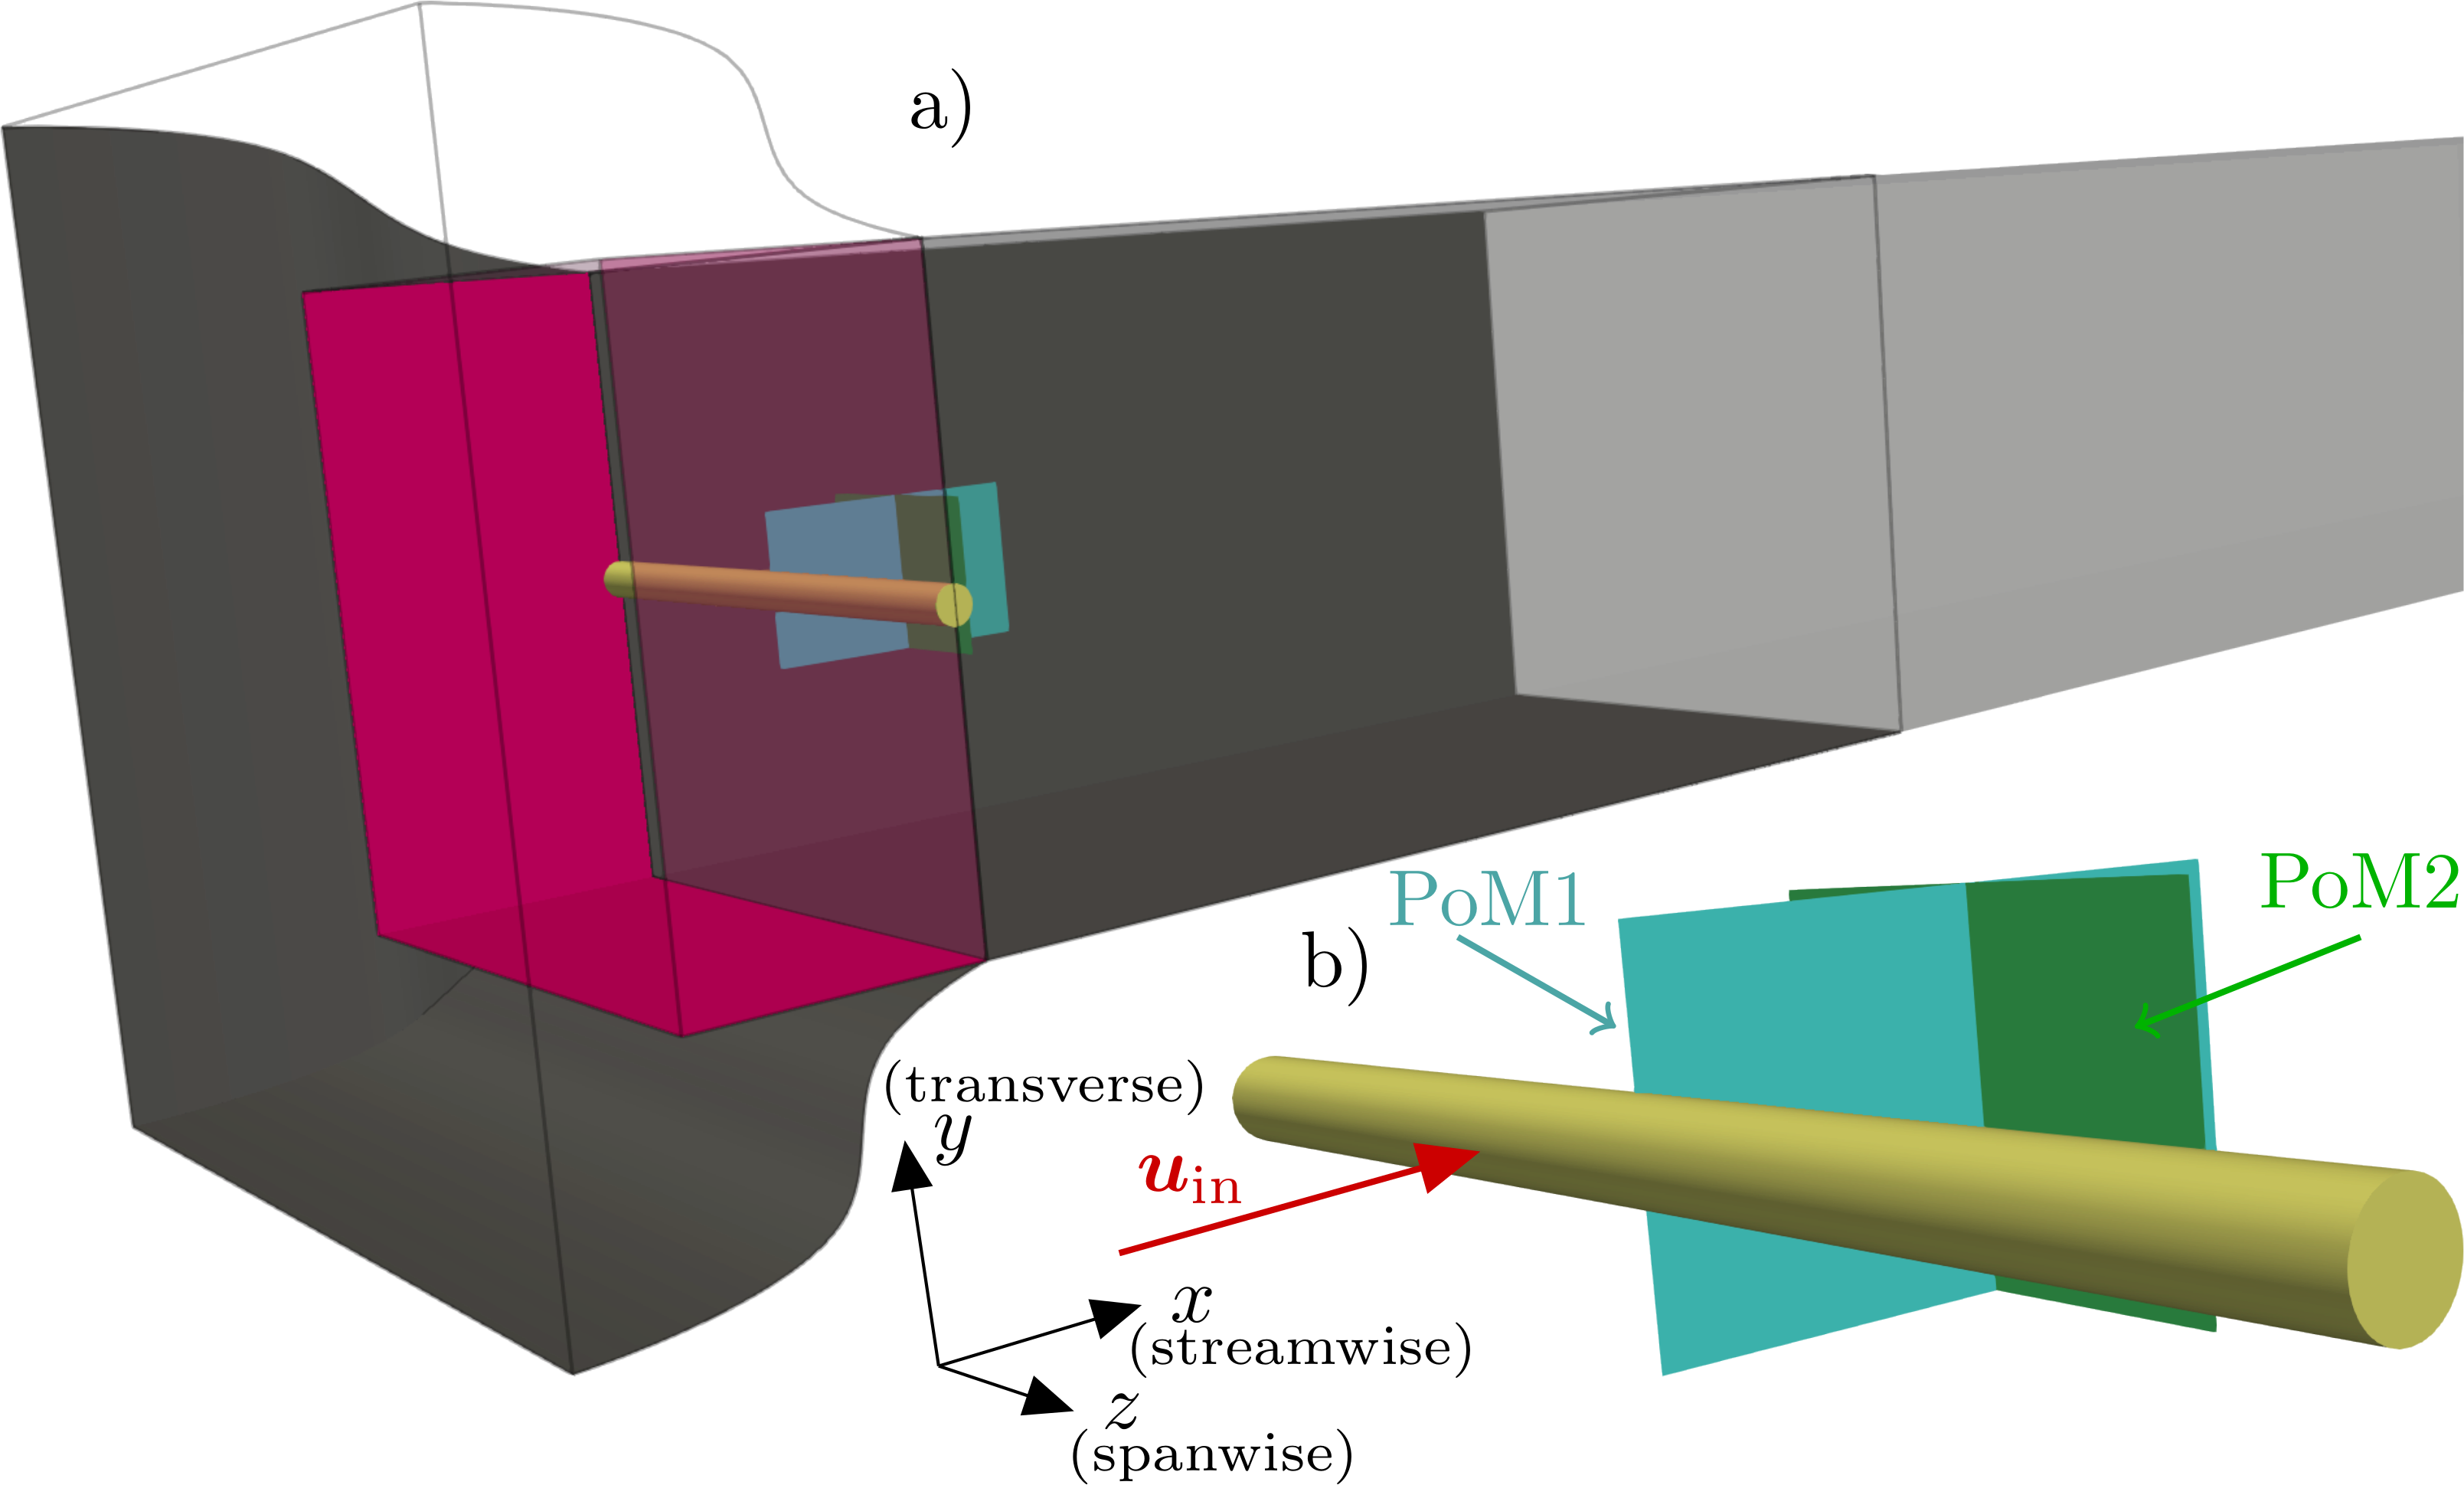
\includegraphics[width=0.98\textwidth]{02_images/00_export/figure1.png}
    \caption{(a) Sketch of the experimental set up and of the corresponding computational domain. Geometrical discrepancy between the two is highlighted in red. The planes of measurement used in experiment are shown in teal (PoM1) and green (PoM2). (b) Detail of the cylinder and planes of measurement.}
    \label{fig:geom}
\end{figure}
The problem at hand consists of the cross-flow around a circular cylinder. The experimental data were measured at a blown-down facility with a closed test section of $250\times 250\,\mathrm{mm}^{2}$. The cylinder model of diameter $d = 15 \,\mathrm{mm}$ and spanning the whole test section was placed at the test section center and oriented transversely with respect to the main flow direction as indicated in Figure~\ref{fig:geom}a. The cross-section blockage caused by the cylinder model was about $6\,\%$.{}

The experimental data on the flow field were obtained via the time-resolved Particle Image Velocimetry (PIV). The measurement apparatus comprises a laser and CMOS cameras by the Dantec company. The used laser is the New Wave Pegasus, Nd:YLF double head with wavelength of $527\, \mathrm{nm}$, maximal frequency $10\, \mathrm{kHz}$, shot energy of $10\, \mathrm{mJ}$ (for $1\, \mathrm{kHz}$) and the corresponding power of $10\, \mathrm{W}$ per one head. The cameras are the Phantom V611 and SpeedSense VEO 410 with the resolution of $1 280 \times 800$ pixels able of acquiring double snaps with frequency up to $3\, \mathrm{kHz}$ (at full resolution). The flow was visualized utilizing the SAFEX particles, i.e. oil droplets $1\,\mu \mathrm{m}$ in diameter. The data were collected and postprocessed in the DynamicStudio software \cite{dynamicsStudio}.

The flow velocity ($\bm{u} = (u,v,w)^{\transp}$) data were sampled for $2\,\mathrm{s}$ with the acquisition frequency of $2\,\mathrm{kHz}$. The data were collected on two planes of measurements (PoM) as depicted in Figure~\ref{fig:geom}b. The stream-wise oriented PoM (PoM1) lies in the $x-y$ plane. Fixing the origin of the problem cartesian coordinate system at the cylinder center of gravity {and scaling the distances by cylinder diameter $d$ as $\bm{x}_{r} = (x_r,y_{r},z_{r}) = (x,y,z)/d = \bm{x}/d$}, PoM1 is defined as 
\begin{equation}
    \label{eq:POM1}
    {\mathrm{PoM1} = \{(x_r,y_r,z_r)\in\mathbb{R}^{3}:x_r\in [0.5,7],\,y_r\in[-2,2],z_r=0\}}\,.
\end{equation}
The PoM2 lies in the $y-z$ plane in the distance of {$x_r = 3.83$} behind the cylinder, i.e. 
\begin{equation}
    \label{eq:POM1}
    {\mathrm{PoM2} = \{(x_r,y_r,z_r)\in\mathbb{R}^{3}:x_r = 3.83,\,y_r\in[-2,2],z_r\in[-3,3]\}}\,.
\end{equation}
In the PoM1, the classical variant of PIV with a single Phantom camera able to evaluate two velocity components ($u$ and $v$) was applied. In the PoM2, the stereo-PIV version with two VEO cameras was utilized and all the three velocity components ($u$, $v$ and $w$) were acquired. The velocities in PoM1 were evaluated in the mesh of {\noteMI{$159\times 99$}} points in the $x$ and $y$ axis direction, respectively. The measurement mesh resolution in PoM2 was {\noteMI{$61\times 91$}} points with respect to the $y$ and $z$ axis directions. A detailed description of the applied PIV system may be found in \cite{prochazka2019}.


The CFD model geometry was as close to the experimental apparatus as possible. In both the experiment and the simulation, the cylinder comes in contact with an almost uniform flow field of mean velocity $\bm{u}_{\mathrm{in}} = (u_{\mathrm{in}},0,0)^{\transp}\,\mathrm{m\,s^{-1}}$, where $u_{\mathrm{in}} = 5\,\mathrm{m\,s^{-1}}$ resulting in the aforementioned Reynolds number of $\Rey = u_{\mathrm{in}}\,d/\nu = 4815$, with $\nu$ being the fluid (air) kinematic viscosity. In the experiment, a flow field with a low turbulence of intensity $I\approx 0.2\,\%$ and a good regularity with departures below $1\,\%$ is provided by an inlet nozzle. The region inside the inlet nozzle has been modeled by a test section extension in the upstream direction to capture the cylinder effect on the upstream flow-field. The modeled test section walls in front of the cylinder were considered as impermeable but not posing any tangential resistance to the flow. As a result, the simulated flow field at the contact with the cylinder was almost uniform, similarly to the experiment. The situation is illustrated in Figure~\ref{fig:geom}a, where the special \textit{virtual walls} of the computational domain are shown in red.

